%%%%%%%%%%%%%%%%%%%%%%%%%%%%%%%%%%%%%%%%%%%%%%%%%%%%%%%%%%%%%%%%%%%%%%
%%  Copyright by Wenliang Du.                                       %%
%%  This work is licensed under the Creative Commons                %%
%%  Attribution-NonCommercial-ShareAlike 4.0 International License. %%
%%  To view a copy of this license, visit                           %%
%%  http://creativecommons.org/licenses/by-nc-sa/4.0/.              %%
%%%%%%%%%%%%%%%%%%%%%%%%%%%%%%%%%%%%%%%%%%%%%%%%%%%%%%%%%%%%%%%%%%%%%%

\newcommand{\commonfolder}{../../common-files}

\documentclass[11pt]{article}

\usepackage[most]{tcolorbox}
\usepackage{times}
\usepackage{epsf}
\usepackage{epsfig}
\usepackage{amsmath, alltt, amssymb, xspace}
\usepackage{wrapfig}
\usepackage{fancyhdr}
\usepackage{url}
\usepackage{verbatim}
\usepackage{fancyvrb}
\usepackage{adjustbox}
\usepackage{listings}
\usepackage{color}
\usepackage{subfigure}
\usepackage{cite}
\usepackage{sidecap}
\usepackage{pifont}
\usepackage{mdframed}
\usepackage{textcomp}
\usepackage{enumitem}


% Horizontal alignment
\topmargin      -0.50in  % distance to headers
\oddsidemargin  0.0in
\evensidemargin 0.0in
\textwidth      6.5in
\textheight     8.9in 

\newcommand{\todo}[1]{
\vspace{0.1in}
\fbox{\parbox{6in}{TODO: #1}}
\vspace{0.1in}
}


\newcommand{\unix}{{\tt Unix}\xspace}
\newcommand{\linux}{{\tt Linux}\xspace}
\newcommand{\minix}{{\tt Minix}\xspace}
\newcommand{\ubuntu}{{\tt Ubuntu}\xspace}
\newcommand{\setuid}{{\tt Set-UID}\xspace}
\newcommand{\openssl} {\texttt{openssl}}


\pagestyle{fancy}
\lhead{\bfseries SEED Labs}
\chead{}
\rhead{\small \thepage}
\lfoot{}
\cfoot{}
\rfoot{}


\definecolor{dkgreen}{rgb}{0,0.6,0}
\definecolor{gray}{rgb}{0.5,0.5,0.5}
\definecolor{mauve}{rgb}{0.58,0,0.82}
\definecolor{lightgray}{gray}{0.90}


\lstset{%
  frame=none,
  language=,
  backgroundcolor=\color{lightgray},
  aboveskip=3mm,
  belowskip=3mm,
  showstringspaces=false,
%  columns=flexible,
  basicstyle={\small\ttfamily},
  numbers=none,
  numberstyle=\tiny\color{gray},
  keywordstyle=\color{blue},
  commentstyle=\color{dkgreen},
  stringstyle=\color{mauve},
  breaklines=true,
  breakatwhitespace=true,
  tabsize=3,
  columns=fullflexible,
  keepspaces=true,
  escapeinside={(*@}{@*)}
}

\newcommand{\newnote}[1]{
\vspace{0.1in}
\noindent
\fbox{\parbox{1.0\textwidth}{\textbf{Note:} #1}}
%\vspace{0.1in}
}


%% Submission
\newcommand{\seedsubmission}{You need to submit a detailed lab report, with screenshots,
to describe what you have done and what you have observed.
You also need to provide explanation
to the observations that are interesting or surprising.
Please also list the important code snippets followed by
explanation. Simply attaching code without any explanation will not
receive credits.}

%% Book
\newcommand{\seedbook}{\textit{Computer \& Internet Security: A Hands-on Approach}, 2nd
Edition, by Wenliang Du. See details at \url{https://www.handsonsecurity.net}.}

%% Videos
\newcommand{\seedisvideo}{\textit{Internet Security: A Hands-on Approach},
by Wenliang Du. See details at \url{https://www.handsonsecurity.net/video.html}.}

\newcommand{\seedcsvideo}{\textit{Computer Security: A Hands-on Approach},
by Wenliang Du. See details at \url{https://www.handsonsecurity.net/video.html}.}

%% Lab Environment
\newcommand{\seedenvironment}{This lab has been tested on our pre-built
Ubuntu 16.04 VM, which can be downloaded from the SEED website. }

\newcommand{\seedenvironmentA}{This lab has been tested on our pre-built
Ubuntu 16.04 VM, which can be downloaded from the SEED website. }

\newcommand{\seedenvironmentB}{This lab has been tested on our pre-built
Ubuntu 20.04 VM, which can be downloaded from the SEED website. }

\newcommand{\seedenvironmentAB}{This lab has been tested on our pre-built
Ubuntu 16.04 and 20.04 VMs, which can be downloaded from the SEED website. }

\newcommand{\nodependency}{Since we use containers to set up the lab environment, 
this lab does not depend too much on our SEED VM. You can do this lab
using other VMs or physical machines. }







\newcommand{\seedlabcopyright}[1]{
\vspace{0.1in}
\fbox{\parbox{6in}{\small Copyright \copyright\ {#1}\ \ by Wenliang Du.\\
      This work is licensed under a Creative Commons
      Attribution-NonCommercial-ShareAlike 4.0 International License.
      If you remix, transform, or build upon the material, 
      this copyright notice must be left intact, or reproduced in a way that is reasonable to
      the medium in which the work is being re-published.}}
\vspace{0.1in}
}






\lhead{\bfseries SEED Labs -- Padding Oracle Attack Lab}

\begin{document}


\begin{center}
{\LARGE Padding Oracle Attack Lab}
\end{center}

\seedlabcopyright{2021}

\newcounter{task}
\setcounter{task}{1}
\newcommand{\tasks} {\bf {\noindent (\arabic{task})} \addtocounter{task}{1} \,}



% *******************************************
% SECTION
% *******************************************
\section{Overview}

The learning objective of this lab is for students to get a hands-on 
experience on an interesting attack on crypto systems. 
Some systems, when decrypting a given ciphertext,
verify whether the padding is valid or not,
and throw an error if the padding is invalid. This
seemly-harmless behavior enables a type of attack
called \textit{padding oracle attack}.
The attack was originally published in 2002 by Serge Vaudenay, and
many well-known systems were found vulnerable to this attack, 
including Ruby on Rails, ASP.NET, and OpenSSL.


In this lab, students are given two oracle servers running inside
a container. Each oracle has a secret message hidden inside,
and it lets you know the ciphertext and the IV, but not the plaintext
or the encryption key. 
You can send a ciphertext (and the IV) to the oracle;
it will decrypt the ciphertext using the encryption key,
and tell you whether the padding is valid or not. 
Your job is to use the response from
the oracle to figure out the content of the secret message. 
This lab covers the following topics:

\begin{itemize}[noitemsep]
\item Secret-key encryption
\item Encryption modes and paddings
\item Padding oracle attack
\end{itemize}


\paragraph{Readings.}
Detailed coverage of the secret-key encryption can be found in the following,
but the padding oracle attack is not covered in the current edition
(future editions will include this attack). Students can find tutorials
on this attack from online resources, such as Wikipedia.

\begin{itemize}
\item Chapter 21 of the SEED Book, \seedbook
\end{itemize}


\paragraph{Lab environment.} \seedenvironmentC


% *******************************************
% SECTION
% *******************************************
\section{Lab Environment}

In this lab, we use a container to run the padding oracle. 


\paragraph{Container Setup and Commands.}
%%%%%%%%%%%%%%%%%%%%%%%%%%%%%%%%%%%%%%%%%%%%
Please download the
\texttt{Labsetup.zip} file to your VM from the lab's website,
unzip it, enter the \texttt{Labsetup} folder, and 
use the \texttt{docker-compose.yml} file to 
set up the lab environment. Detailed explanation
of the content in this file and all the involved 
\texttt{Dockerfile} can be found from the 
user manual, which is linked to the website of this lab.
If this is the first time you set up a SEED lab environment
using containers, it is very important that you read 
the user manual. 

In the following, we list some of the commonly
used commands related to Docker and Compose. 
Since we are going to use 
these commands very frequently, we have created aliases for them
in the \texttt{.bashrc} file (in our provided SEEDUbuntu 20.04 VM).


\begin{lstlisting}
$ docker-compose build  # Build the container image
$ docker-compose up     # Start the container
$ docker-compose down   # Shut down the container

// Aliases for the Compose commands above
$ dcbuild       # Alias for: docker-compose build
$ dcup          # Alias for: docker-compose up
$ dcdown        # Alias for: docker-compose down
\end{lstlisting}


All the containers will be running in the background. To run
commands on a container, we often need to get a shell on
that container. We first need to use the \texttt{"docker ps"}  
command to find out the ID of the container, and then
use \texttt{"docker exec"} to start a shell on that 
container. We have created aliases for them in
the \texttt{.bashrc} file.

\begin{lstlisting}
$ dockps        # Alias for: docker ps --format "{{.ID}}  {{.Names}}" 
$ docksh <id>   # Alias for: docker exec -it <id> /bin/bash

# The following example shows how to get a shell inside hostC
$ dockps
b1004832e275  hostA-10.9.0.5
0af4ea7a3e2e  hostB-10.9.0.6
9652715c8e0a  hostC-10.9.0.7

$ docksh 96
root@9652715c8e0a:/#  

# Note: If a docker command requires a container ID, you do not need to 
#       type the entire ID string. Typing the first few characters will 
#       be sufficient, as long as they are unique among all the containers. 
\end{lstlisting}


If you encounter problems when setting up the lab environment, 
please read the ``Common Problems'' section of the manual
for potential solutions.


%%%%%%%%%%%%%%%%%%%%%%%%%%%%%%%%%%%%%%%%%%%%


% *******************************************
% SECTION
% *******************************************
\section{Task 1: Getting Familiar with Padding}

For some block ciphers, when the size of a plaintext is not a multiple
of the block size, padding may be required.
The PKCS\#5 padding scheme is widely used by many block
ciphers (see Chapter 21.4 of the SEED book for details).
We will conduct the following experiments to
understand how this type of padding works.

We can use the \texttt{"echo -n"} command to create a file.
The following example
creates a file \texttt{P} with length 5 (without the \texttt{-n} option, the length will
be 6, because a newline character will be added by \texttt{echo}):

\begin{lstlisting}
$ echo -n "12345" > P
\end{lstlisting}

We use \texttt{"openssl enc -aes-128-cbc -e"} to encrypt this file
using 128-bit AES with CBC mode.
To see what is added to the padding during the encryption, 
we will decrypt the ciphertext using \texttt{"openssl enc -aes-128-cbc -d"}.
Unfortunately, decryption by default will automatically remove the padding, making it
impossible for us to see the padding. However, the command does have an option called
\texttt{"-nopad"}, which disables the padding, i.e., during the decryption, the command will not
remove the padded data. Therefore, by looking at the decrypted
data, we can see what data are used in the padding.

\begin{lstlisting}
$ openssl enc -aes-128-cbc -e -in P -out C
$ openssl enc -aes-128-cbc -d -nopad -in C -out P_new
\end{lstlisting}

It should be noted that padding data may not be printable, so you need to
use a hex tool to display the content. The following example shows
how to display a file in the hex format:

\begin{lstlisting}
$ xxd P_new
00000000: 3132 3334 350b 0b0b 0b0b 0b0b 0b0b 0b0b  12345...........
\end{lstlisting}

Your job is to create three files, which contain 5 bytes, 10 bytes, and 16 bytes, respectively.
Using the method above, please figure out what paddings are added to the three files.



% *******************************************
% SECTION
% *******************************************
\section{Task 2: Padding Oracle Attack (Level 1)}

Some systems, when decrypting a given ciphertext,
verify whether the padding is valid or not,  
and throw an error if the padding is invalid. This 
seemly-harmless behavior enables a type of attack 
called \textit{padding oracle attack}.
The attack was originally published in 2002 by Serge Vaudenay, and 
many well-known systems were found vulnerable to this type of 
attacks, including Ruby on Rails, ASP.NET, and OpenSSL. 



% -------------------------------------------
% SUBSECTION
% -------------------------------------------
\subsection{The Oracle Setup} 

In this task, we provide a padding oracle hosted on port \texttt{5000}.
The oracle has a secret message inside, and it 
prints out the ciphertext of this secret message. The encryption algorithm
and mode used is AES-CBC, and the encryption key is \texttt{K}, which
is unknown to others.
You can interact with the oracle using \texttt{"nc 10.9.0.80 5000"}.
You will see the following hexadecimal data provided by the oracle. 
The first 16 bytes is the IV, and the rest is the ciphertext. 
From the length, you can see that the ciphertext has 32 bytes, i.e.,
2 blocks, but the actual length of the plaintext is unknown
due to the padding. 

\begin{lstlisting}
$ nc 10.9.0.80 5000
01020304050607080102030405060708a9b2554b094411...
\end{lstlisting}

The oracle accepts input from you. The format of the input 
is the same as the message above: 16-bytes of the IV, concatenated
by the ciphertext. The oracle will decrypt the ciphertext using 
its own secret key \texttt{K}  and the IV provided by you.
It will not tell you the plaintext, but
it does tell you whether the padding is valid or not. 
Your task is to use the information provided by the oracle
to figure out the actual content of the secret message. 
For the sake of simplicity, you only need to find out one block
of the secret message. For the debugging purpose,
we provide the secret message in the following (it is 
in the source code of the oracle).

\begin{lstlisting}[language=c++]
static std::array<unsigned char, 29> PLAIN_TEXT = {
    0x11, 0x22, 0x33, 0x44, 0x55, 0x66, 0x77, 0x88,
    0x11, 0x22, 0x33, 0x44, 0x55, 0x66, 0x77, 0x88,
    0x11, 0x22, 0x33, 0x44, 0x55, 0x66, 0x77, 0x88,
    0xaa, 0xbb, 0xcc, 0xdd, 0xee
};
\end{lstlisting}
 
The secret message is provided only for debugging purposes, and you cannot assume that 
you know this message.  You need to use the 
padding oracle attack to derive this message; you need to 
show your steps. 

% -------------------------------------------
% SUBSECTION
% -------------------------------------------
\subsection{Deriving the Plaintext Manually} 


The objective of this task is to figure out the plaintext 
of the secret message. It has two blocks P1 and P2. 
We only need to get P2 (getting P1 is similar). 
We have provided a skeleton code called \texttt{manual\_attack.py}. 
You can use this as a basis to construct your attack. We 
will explain each piece of this code. 


First, let's get the ciphertext from the oracle. 
The ciphertext in this task consists of two blocks, and 
we use two 16-byte bytearrays \texttt{C1} and \texttt{C2}
to hold the content of these two blocks.

\begin{lstlisting}[language=python]
oracle = PaddingOracle('127.0.0.1', 5000)

# Get the IV + Ciphertext from the oracle
iv_and_ctext = bytearray(oracle.ctext)
IV    = iv_and_ctext[00:16]
C1    = iv_and_ctext[16:32]  # 1st block of ciphertext
C2    = iv_and_ctext[32:48]  # 2nd block of ciphertext

print("C1:  " + C1.hex())
print("C2:  " + C2.hex())
\end{lstlisting}


\begin{figure}[htb]
  \begin{center}
    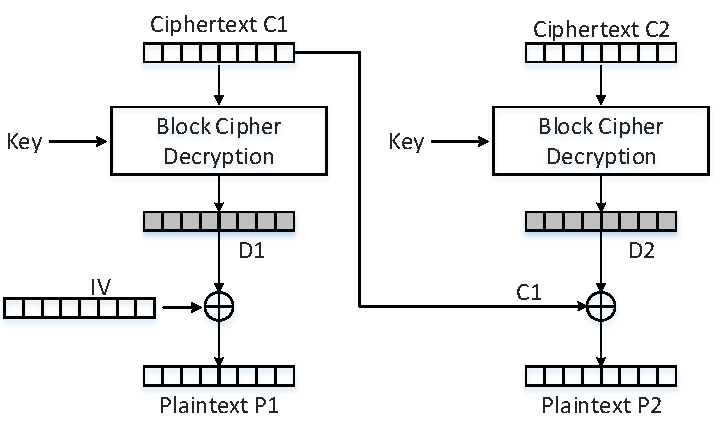
\includegraphics[width=0.6\textwidth]{Figs/cbc-dec.pdf}
  \end{center}
  \caption{Decryption using CBC}
  \label{fig:cbc-dec}
\end{figure}
 
 
As depicted in Figure~\ref{fig:cbc-dec}, D1 and D2 are the 
output of the AES block cipher. If we can 
get their values, we can easily get the plaintext
by xoring them with the ciphertext (or IV for the first block). 
In this task, we focus on the second block P2. Therefore, if we can
figure out the values of D2, 
we can calculate P2 using P2 = C1 $\oplus$ D2.


We will not explain the details of the padding oracle attack
in this lab description. Students can find the details from
online resources, such as Wikipedia (the current SEED book does not 
cover this attack).  The general idea of the attack
is to send to the oracle a ciphertext with modified 
C1 (let's call it CC1). Although the oracle will not tell us the result 
of D2 $\oplus$ CC1, it does tell us whether the result
has a valid padding or not. That opens the door 
for us to figure out the value of D2. 

There are 16 bytes in D2, we can figure out its value one 
byte at a time. In the skeleton code, we have initialized
two arrays D2 and CC1. Their initial values do not really matter.
Your task is to use an iterative process to figure 
out the value for the D2 array. For each iteration, you need 
to construct the CC1 array properly. 

\begin{lstlisting}[language=python]
# The inital value of D2 does not matter. Our job is to 
# find its correct values. 
D2 = bytearray(16)

D2[0]  = C1[0]
D2[1]  = C1[1]
...
D2[15] = C1[15]

# CC1 is used to replace the C1 block in the ciphertext
# Its values need to be set properly in each round
CC1 = bytearray(16)

CC1[0]  = 0x00
CC1[1]  = 0x00
...
CC1[15] = 0x00
\end{lstlisting}

In each iteration, we focus on one byte of CC1.
We try all 256 possible values for that byte, and send the constructed
ciphertext CC1 + C2 (plus the IV) to the oracle, and see
which value makes the padding valid.
As long as our construction is correct, there will be
one valid value. This value helps us get one byte of D2.
The code in the following focuses on K=1. It can 
help us find the value for D[15].

\begin{lstlisting}[language=python]
K = 1
for i in range(256):
      CC1[16 - K] = i
      status = oracle.decrypt(IV + CC1 + C2)
      if status == "Valid":
          print("Valid: i = 0x{:02x}".format(i))
          print("CC1: " + CC1.hex())
\end{lstlisting}
 
You can use the skeleton code as your basis, manually
change the value of K, use the execution result in
each round to set the D2 accordingly, and then
re-run the program with a updated CC1
to get the next byte of D2, i.e., D2[14]. 
Repeating the step, you can get D2[13], D2[12], ..., D2[0].
Once you get the entire D2, you get the value of the plaintext P2. 

\begin{lstlisting}[language=python]
# Once you get all the 16 bytes of D2, you can easily get P2
P2 = xor(C1, D2)
print("P2:  " + P2.hex())
\end{lstlisting}
 
\paragraph{Note.} Figuring out all the 16 bytes of D2 may be too
tedious. Students can stop after getting 6 bytes of D2. That will 
unlock the last 6 bytes of the plaintext P2 (including
the padding). It is sufficient. 
Although students can write code to automate the entire process, it is the 
intention of the lab to force students to do it manually. 
Therefore, the lab report needs to include how each byte (for at least 6 bytes) 
of D2 is obtained. 
In the next task, students will be required to automate this process. 


% *******************************************
% SECTION
% *******************************************
\section{Task 3: Padding Oracle Attack (Level 2)}


We did manual attacks in the previous task. In this task,
we will automate the attack process, and this time, we 
need to get all the blocks of the plaintext. When the 
container starts, two padding oracle servers will be started, one for the 
Level-1 task, and the other is for the Level-2 task, i.e.,
this task. The Level-2 server listens to port \texttt{6000}. 
Although the key and the secret message are in the 
binary code of the oracle program, we have tried to 
obfuscate them, so it will not be very easy to 
find them from the binary. Moreover, learning the secret
message does not help the padding oracle attack at all. Students'
grade depends on how they derive the secret message using
the padding oracle attack, not on whether they know the secret message
or not.


It should be noted that every time you make a new connection to the 
oracle, the oracle will generate a new key and IV to encrypt the 
secret message (the message is still the same). That is why
you will see a different ciphertext. 
However, if you stay inside an existing connection, 
the key and IV will not change. 


You can write a program to derive all the blocks
of the secret message in one run, but 
you are allowed to write your program to get one block 
at a time. Eventually, you need to print out all the 
blocks. In your report, you need to include your code, along with 
the screenshots of the execution results. 



% *******************************************
% SECTION
% *******************************************
\section{Submission}

%%%%%%%%%%%%%%%%%%%%%%%%%%%%%%%%%%%%%%%%

You need to submit a detailed lab report, with screenshots,
to describe what you have done and what you have observed.
You also need to provide explanation
to the observations that are interesting or surprising.
Please also list the important code snippets followed by
explanation. Simply attaching code without any explanation will not
receive credits.

%%%%%%%%%%%%%%%%%%%%%%%%%%%%%%%%%%%%%%%%



% *******************************************
% SECTION
% *******************************************
\section{Acknowledgment}

We would like to acknowledge the contribution made by the following people and organizations:

\begin{itemize}
\item Jiamin Shen developed the following: the code running inside the container, 
      the initial version of the padding oracle attack task. 

\item The US National Science Foundation provided the funding for the SEED project from 2002 
      to 2020.

\item Syracuse University provided the resources for the SEED project from 2001 onwards.
\end{itemize}




\end{document}
%%%%%%%%%%%%%%%%%%%%%%%%%%%%%%%%%%%%%%%%%%%%%%%%%%%%%%%%%%%%%%%%%%%%%
%%%%%%%%%%%%%%%%%%%%%%%%%%%%%%%%%%%%%%%%%%%%%%%%%%%%%%%%%%%%%%%%%%%%%


